\documentclass[11pt,a4paper]{article}
\usepackage[utf8]{inputenc}
\usepackage[italian]{babel}
\usepackage{geometry}
\geometry{a4paper, margin=2.5cm}
\usepackage{graphicx}
\usepackage{booktabs}
\usepackage{amsmath}
\usepackage{hyperref}
\usepackage{cite}

% Impostazioni dei link cliccabili
\hypersetup{
    colorlinks=true,
    linkcolor=blue,
    filecolor=magenta,      
    urlcolor=cyan,
    pdftitle={Relazione Finale Data Science},
}

\title{\textbf{Analisi Predittiva del Customer Churn}\\
\large Progetto del corso di Introduzione al Pensiero Computazionale e alla Data Science}
\author{Ederone Aurora, Querqui Chiara, Giovannini Stefano \small (Gruppo 13) \\ Università di Bologna}
\date{Anno Accademico 2025/2026}
\begin{document}

\maketitle

\section{Introduzione}
Nel mercato delle telecomunicazioni la fidelizzazione della clientela rappresenta una delle sfide strategiche più rilevanti per la sostenibilità economica delle imprese. In questo contesto, il fenomeno del \textit{customer churn}, ovvero l'abbandono del servizio da parte di un utente a favore di un concorrente, comporta non solo una perdita diretta in termini di fatturato corrente, ma anche un incremento dei costi operativi legati all'acquisizione di nuova clientela.

L'obiettivo di questo progetto è realizzare un flusso di lavoro completo e riproducibile di Data Science per analizzare un dataset aziendale di telecomunicazioni e addestrare modelli predittivi capaci di identificare i clienti a maggior rischio di abbandono. L'attività si è articolata in sei fasi logiche: l'impostazione del sistema di versionamento del codice (Git), lo screening della qualità dei dati, un'analisi esplorativa approfondita supportata da visualizzazioni grafiche, la preparazione delle feature, l'addestramento comparativo di algoritmi lineari e non lineari ed, infine, una valutazione critica basata su metriche idonee.

Tutto il codice sorgente, il notebook di sviluppo operativo sulla piattaforma Google Colab e i file di configurazione necessari alla riproducibilità dell'analisi sono consultabili presso la repository GitHub del team al seguente indirizzo: 
\url{https://github.com/auroraederone/Progetto-Data-Science}.


\section{Dataset e Qualità dei Dati}
Il dataset preso in esame, denominato \textit{Customer Churn}, si compone inizialmente di un campione di $7.043$ osservazioni distribuite su $21$ variabili descrittive, le quali racchiudono informazioni di natura anagrafica (come genere, presenza di partner o dipendenti), caratteristiche contrattuali e tecnologiche (come tipologia di connessione internet, servizi di supporto attivi) e metriche economiche di utilizzo del servizio (spesa mensile e spesa totale complessiva). 

\subsection{Analisi della Qualità}
Durante la fase preliminare di screening e controllo della qualità dei dati, l'ispezione standard dei valori mancanti tramite funzioni automatizzate non ha rilevato valori nulli; tuttavia, conducendo una ricerca più approfondita volta ad identificare \textit{missing values} nascosti (ovvero celle composte da stringhe vuote o spazi), è emersa un'anomalia strutturale all'interno della variabile \texttt{TotalCharges}, la quale presentava $11$ record vuoti. 

Un'analisi contestuale di questi specifici record ha evidenziato che l'anomalia non era frutto di un errore casuale di trascrizione del database, bensì una conseguenza logica: tutti gli $11$ clienti presentavano un valore di \texttt{Tenure} (anzianità di servizio espresso in mesi) pari a zero; un utente appena contrattualizzato non può logicamente aver accumulato uno storico di spesa. Pertanto, per evitare di introdurre distorsioni arbitrarie sostituendo i dati mancanti con la media o la mediana, si è optato per la rimozione  di queste osservazioni; questa operazione ha ridotto il campione a $7.032$ osservazioni totali, a fronte di una perdita di dati trascurabile (inferiore allo $0.2\%$).

Al fine di escludere la presenza di anomalie o valori estremi che avrebbero potuto disturbare l'addestramento degli algoritmi, è stato applicato alle variabili numeriche il metodo statistico dell'Intervallo Interquartile ($IQR$), espresso dalla seguente relazione matematica:
\begin{equation*}
    IQR = Q_3 - Q_1
\end{equation*}
I limiti di tolleranza calcolati hanno confermato l'assenza totale di outlier nelle metriche chiave del dataset; inoltre, il controllo della cardinalità delle variabili qualitative ha evidenziato una struttura pulita e a bassa dimensionalità.

\subsection{Riflessione su Class Imbalance}
L'evidenza statistica più critica emersa in questa fase riguarda la distribuzione della variabile target binaria \texttt{Churn}. Il dataset ripulito evidenzia che il $73.42\%$ dei clienti ($5.163$ osservazioni) non ha abbandonato l'azienda (\texttt{Churn = No}), mentre solo il $26.58\%$ ($1.869$ osservazioni) appartiene alla classe dei clienti che hanno rescisso il contratto (\texttt{Churn = Yes}). 

Questo forte sbilanciamento delle classi (\textit{Class Imbalance}) costituisce un vincolo per la successiva fase di modellazione predittiva. Gli algoritmi di Machine Learning tendono di base a massimizzare l'accuratezza globale focalizzandosi sulla classe maggioritaria e, di conseguenza, una metrica basata unicamente sull'Accuracy risulterebbe ingannevole: un modello che predice sistematicamente \texttt{No} per qualsiasi utente otterrebbe un'accuratezza del $73.42\%$, pur fallendo totalmente l'obiettivo di intercettare i clienti a rischio. Per questo motivo, nelle fasi successive utilizzeremo metriche adatte a dati sbilanciati, valutando i modelli soprattutto attraverso l'F1-Score e la Recall sulla classe minoritaria.

\section{Analisi Esplorativa e Visualizzazione}
L'obiettivo fondamentale dell'analisi esplorativa dei dati è quello di abbandonare un approccio tabellare per mappare, descrivere e comprendere le relazioni esistenti tra le diverse variabili esplicative e la variabile target \texttt{Churn}. Per evitare il rischio di trarre conclusioni basate su soli conteggi assoluti, l'intera analisi è stata condotta analizzando il \textit{churn rate}, ovvero la percentuale di clienti che hanno abbandonato il servizio all'interno di ciascuna specifica categoria.

L'indagine è stata guidata dalla formulazione e dalla successiva verifica empirica di quattro ipotesi di ricerca principali:
\begin{enumerate}
    \item \textbf{Impatto della stabilità contrattuale:} è stato ipotizzato che la tipologia di contratto sottoscritto influenzi significativamente la propensione all'abbandono. L'analisi ha confermato questa ipotesi: i clienti con un contratto mensile (\textit{Month-to-month}) presentano un tasso di churn più elevato rispetto a coloro che hanno sottoscritto vincoli annuali o biennali. La stabilità contrattuale agisce quindi come un fattore di ritenzione.
    
    \item \textbf{Fidelizzazione e anzianità (Tenure):} si è ipotizzato che i clienti più recenti, avendo una relazione meno consolidata con l'azienda, mostrino una minore fidelizzazione. Il controllo della distribuzione della variabile \texttt{tenure} tramite boxplot ha convalidato l'ipotesi: la distribuzione dei mesi di anzianità per la classe \texttt{Churn = Yes} si concentra su valori bassi, confermando che il rischio di abbandono è massimo durante i primi mesi di vita del cliente.
    
    \item \textbf{Pressione economica (Monthly Charges):} la terza ipotesi prevedeva che tariffe mensili più elevate agissero come un fattore di spinta all'abbandono. L'analisi distributiva ha evidenziato che i clienti che abbandonano il servizio si concentrano prevalentemente nella fascia medio-alta dei costi mensili, suggerendo una sensibilità della clientela rispetto al prezzo o alla percezione del valore ricevuto.
    
    \item \textbf{Ruolo dei servizi di supporto aggiuntivi:} infine, si è ipotizzato che l'assenza di servizi di assistenza e protezione fosse associata a un churn più elevato. L'analisi incrociata ha dimostrato che i clienti privi di servizi quali \texttt{TechSupport} e \texttt{OnlineSecurity} registrano tassi di abbandono nettamente superiori rispetto a chi ne beneficia.
\end{enumerate}


\subsection{Analisi delle Interazioni e della Multicollinearità}
L'evidenza empirica secondo cui sia l'assenza di \texttt{TechSupport} sia quella di \texttt{OnlineSecurity} fossero associate a un forte incremento del churn ha sollevato un dubbio metodologico, ovvero comprendere se tali variabili rappresentassero scelte d'acquisto speculari (e ridondanti) o comportamenti indipendenti. Per fare chiarezza, è stata calcolata la correlazione lineare di Pearson previa ricodifica numerica delle feature; il coefficiente ha restituito un valore pari a $0.3545$, evidenziando una correlazione positiva debole-moderata. Sebbene sussista una parziale tendenza ad associare i due servizi di protezione, la maggior parte della clientela compie scelte d'acquisto separate; le due variabili contengono quindi un apporto informativo distinto e possono essere mantenute nel dataset senza rischi di ridondanza.

Un quadro fondamentale sulle dinamiche multivariate è emerso dall'analisi della matrice di correlazione complessiva sulle variabili quantitative (vedi Figura \ref{fig:heatmap}), i cui coefficienti lineari offrono spunti importanti per la fase di modellazione:
\begin{itemize}
    \item \textbf{Tenure e Churn ($-0.35$):} rappresenta la relazione lineare più significativa riscontrata con il target. Il segno negativo formalizza una proporzionalità inversa: al crescere dei mesi di fedeltà dell'utente, la propensione all'abbandono diminuisce in modo sensibile, corroborando la teoria della fidelizzazione temporale.
    \item \textbf{Monthly Charges e Churn ($+0.19$):} il coefficiente positivo conferma che l'entità delle tariffe mensili agisce come un fattore di spinta verso la concorrenza.
    \item \textbf{TotalCharges e Churn ($-0.20$):} il segno negativo, apparentemente controintuitivo se confrontato con l'effetto dei costi mensili, è spiegato dal fatto che la spesa totale accumulata è trainata dalla permanenza storica del cliente; i clienti con spese totali molto elevate sono, per definizione, clienti storici e quindi stabilizzati.
\end{itemize}

L'evidenza metodologica più rilevante emersa dalla heatmap riguarda tuttavia la correlazione lineare estremamente elevata tra \texttt{Tenure} e \texttt{TotalCharges}, pari a $+0.83$. Questa forte sovrapposizione, nota come \textit{multicollinearità}, costituisce un elemento di attenzione per gli algoritmi di Machine Learning. Sebbene non rappresenti un problema per i modelli non lineari basati su alberi decisionali, la presenza di variabili così fortemente correlate può destabilizzare il calcolo e l'interpretabilità dei coefficienti nei modelli lineari (come la Regressione Logistica), un aspetto che richiederà una verifica dedicata in fase di valutazione dei risultati.

 \begin{figure}[htbp]
     \centering
    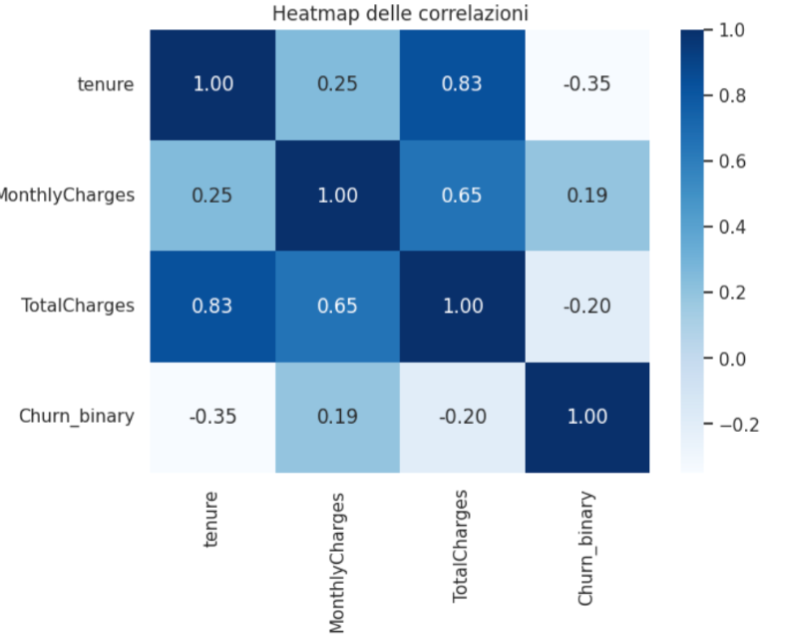
\includegraphics[width=0.7\textwidth]{Images/heatmap_correlazioni.png}
     \caption{Matrice di correlazione lineare di Pearson tra le variabili numeriche e il target di Churn.}
     \label{fig:heatmap}
 \end{figure}


\section{Metodologia e Modellazione}
Una volta consolidata la struttura del dataset e comprese le relazioni principali tra le feature, si è proceduto alla fase di preparazione delle variabili e alla strutturazione del flusso di modellazione predittiva; questa fase mira a trasformare il dataset pulito in una matrice di input idonea agli algoritmi di classificazione, garantendo l'assenza di distorsioni metodologiche.

\subsection{Preparazione del Dataset}
Il flusso di preparazione dei dati si è articolato nei seguenti passaggi sequenziali ed essenziali:
\begin{itemize}
    \item \textbf{Rimozione degli identificativi:} la colonna \texttt{CustomerID} è stata eliminata dal dataset poiché, trattandosi di un codice identificativo univoco, non apporta alcun valore informativo e avrebbe introdotto esclusivamente rumore strutturale nell'addestramento dei modelli.
    \item \textbf{Codifica del target:} la variabile target \texttt{Churn} è stata mappata in formato numerico binario, assegnando il valore $0$ alla classe \texttt{No} (clienti fidelizzati) e il valore $1$ alla classe \texttt{Yes} (clienti che abbandonano); le restanti variabili categoriche qualitative sono state convertite in variabili numeriche binarie tramite la tecnica del \textit{One-Hot Encoding} (\texttt{pd.get\_dummies}). L'impostazione del parametro \texttt{drop\_first=True} ha permesso di escludere la creazione di colonne ridondanti, riducendo il rischio di multicollinearità per i modelli lineari; questa trasformazione ha portato le dimensioni finali della matrice delle feature a $30$ colonne complessive.
    \item \textbf{Train/Test Split Stratificato:} il dataset è stato suddiviso assegnando l'80\% delle osservazioni al training set (pari a $5.625$ record), finalizzato all'addestramento dei modelli, e il restante 20\% al test set ($1.407$ record), dedicato alla valutazione indipendente delle performance; la separazione è stata vincolata tramite una strategia di stratificazione (\texttt{stratify=y}), che ha permesso di mantenere l'esatta proporzione del $26.6\%$ di clienti \textit{churner} sia nell'insieme di addestramento sia in quello di verifica.
    \item \textbf{Feature Scaling e Prevenzione del Data Leakage:} modelli basati su metriche di distanza geometrica o regolarizzazioni lineari risultano fortemente sensibili alla disparità degli ordini di grandezza delle variabili; per questo motivo, si è applicata una procedura di standardizzazione tramite \texttt{StandardScaler}. Per scongiurare fenomeni di \textit{data leakage}, ovvero l'interferenza di informazioni del test set nella fase di addestramento, lo scaler è stato calcolato (\texttt{fit\_transform}) esclusivamente sulla matrice di training e successivamente applicato (\texttt{transform}) alla matrice di test.
\end{itemize}

\subsection{Selezione dei Modelli di Predizione}
Sono stati selezionati e confrontati tre differenti algoritmi di classificazione, bilanciando approcci lineari e non lineari per catturare diversi pattern relazionali nei dati:
\begin{enumerate}
    \item \textbf{Regressione Logistica (Modello Lineare):} scelta per la sua interpretabilità, definisce il confine di separazione tra le classi mediante una combinazione lineare delle feature regolate da una funzione sigmoidea.
    \item \textbf{k-Nearest Neighbors (Modello Non Lineare):} algoritmo basato sulle distanze geometriche nello spazio multidimensionale, classifica un'osservazione in base alla maggioranza dei voti dei suoi \textit{k} vicini più prossimi.
    \item \textbf{Random Forest (Modello Non Lineare):} algoritmo d'insieme (\textit{ensemble}) basato su un'architettura di \textit{n} alberi decisionali indipendenti, capace di catturare interazioni non lineari complesse e robuste rispetto all'overfitting.
\end{enumerate}


\section{Risultati}
Dopo aver addestrato i modelli sui dati standardizzati del training set, ne abbiamo valutato le prestazioni sul test set; per ciascun classificatore sono state estratte le metriche di Accuracy, Precision, Recall e F1-Score riferite alla classe positiva (\texttt{Churn = Yes}), i cui valori sintetici sono esposti nella Tabella \ref{tab:metriche}.


\begin{table}[htbp]
    \centering
    \caption{Quadro comparativo delle metriche di performance sul test set (ordinate per F1-Score).}
    \label{tab:metriche}
    \begin{tabular}{lcccc}
        \hline
        \textbf{Modello} & \textbf{Accuracy} & \textbf{Precision} & \textbf{Recall} & \textbf{F1-Score} \\ \hline
        Regressione Logistica & 0.8038 & 0.6476 & 0.5749 & 0.6091 \\ 
        Random Forest & 0.7882 & 0.6234 & 0.5134 & 0.5630 \\ 
        k-NN & 0.7534 & 0.5362 & 0.5348 & 0.5355 \\ \hline
    \end{tabular}
\end{table}

\subsection{Analisi Comparativa delle Performance}
Dall'analisi comparativa emerge che la \textbf{Regressione Logistica} supera gli approcci non lineari su ogni singola metrica esaminata, registrando un F1-Score di $0.6091$ e un'Accuracy del $80.38\%$. Il Random Forest si attesta in seconda posizione (F1-Score: $0.5630$), mentre il k-NN si dimostra il modello meno efficace nel contesto analizzato. 

Per comprendere la natura di queste discrepanze e valutare l'impatto operativo dei modelli, è necessario analizzare la scomposizione degli errori tramite le rispettive matrici di confusione, visualizzate in Figura \ref{fig:confusion_matrices}. 


\begin{figure}[htbp]
    % --- Prima Matrice ---
    \begin{minipage}[b]{0.32\textwidth}
        \centering
        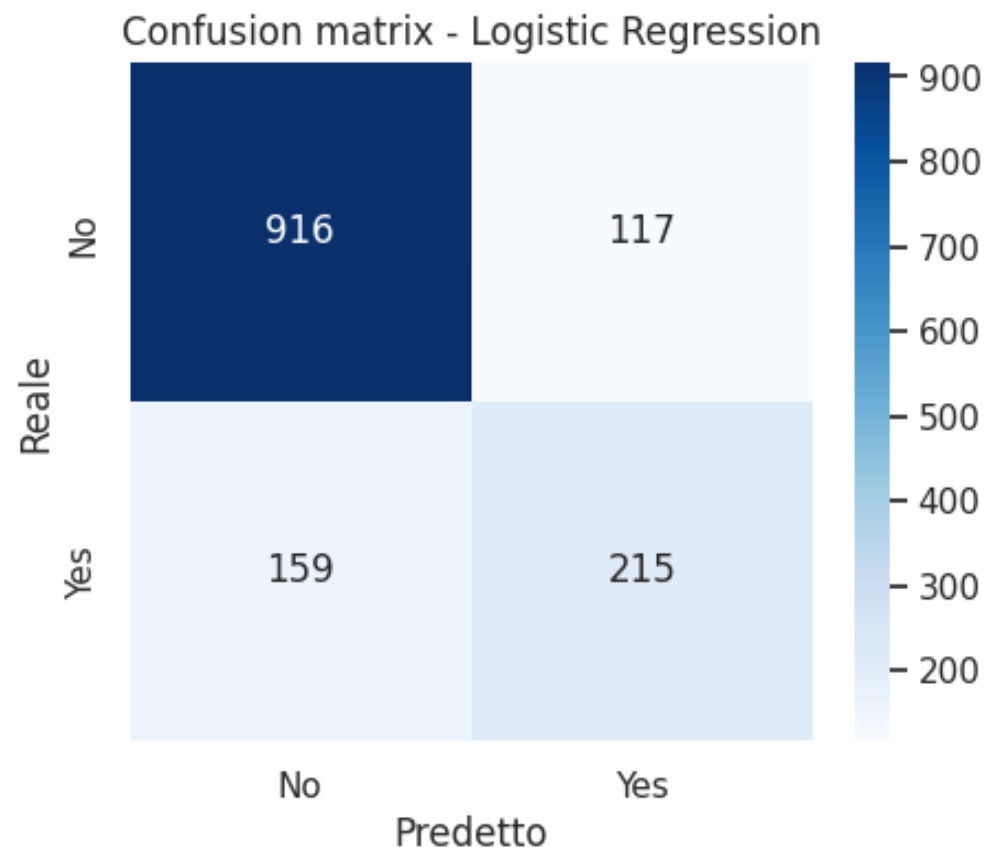
\includegraphics[width=\textwidth]{Images/logistic_regression.png}
        \vspace{1mm} % Crea un piccolo spazio uniforme tra l'immagine e la scritta
        \small a) Regressione Logistica
    \end{minipage}\hfill
    % --- Seconda Matrice ---
    \begin{minipage}[b]{0.32\textwidth}
        \centering
        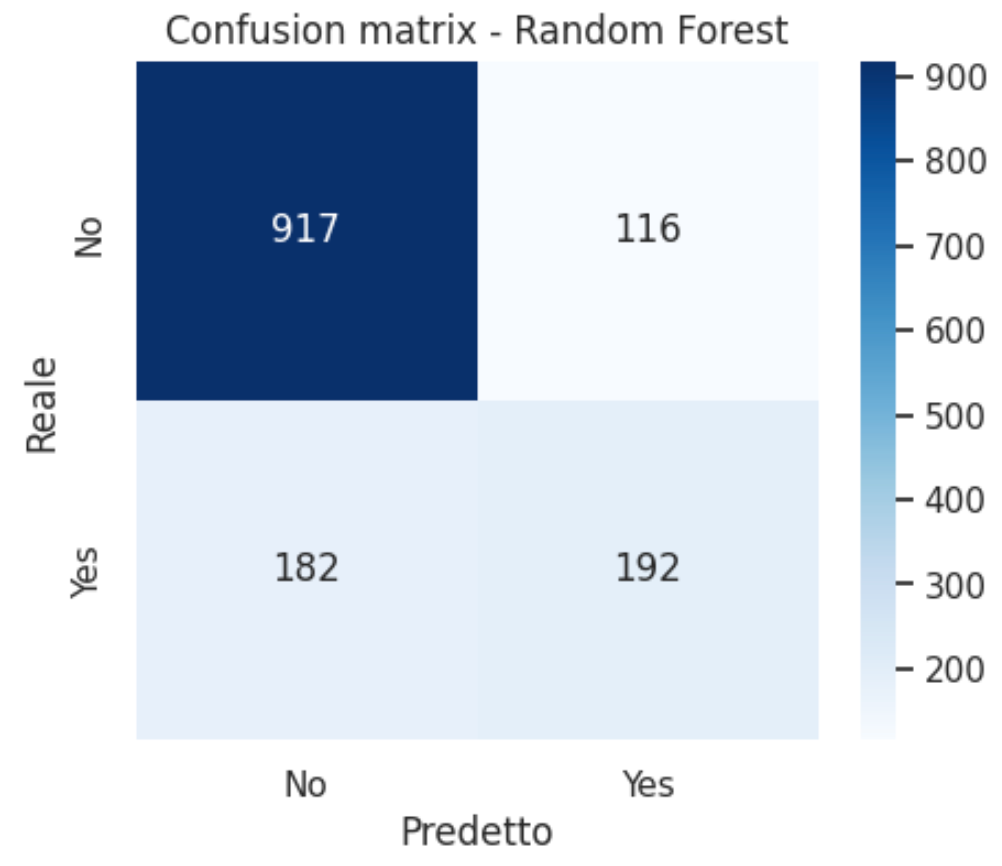
\includegraphics[width=\textwidth]{Images/random_forest.png}
        \vspace{1mm}
        \small b) Random Forest
    \end{minipage}\hfill
    % --- Terza Matrice ---
    \begin{minipage}[b]{0.32\textwidth}
        \centering
        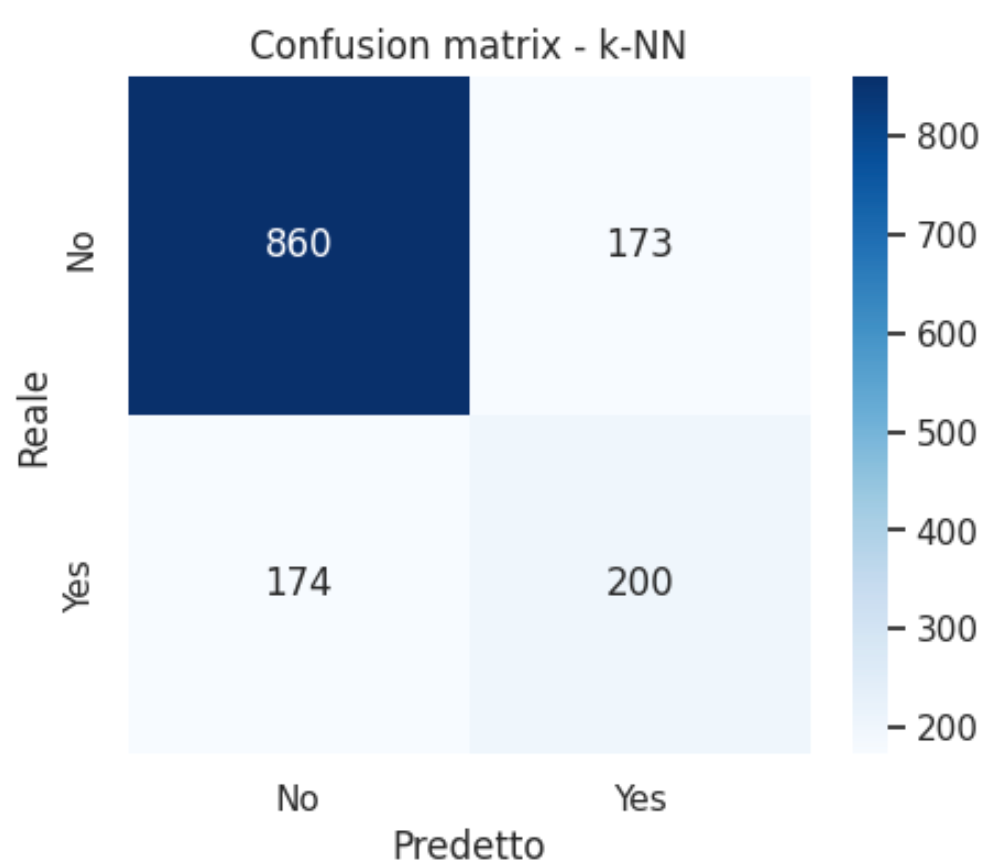
\includegraphics[width=\textwidth]{Images/knn.png}
        \vspace{1mm}
        \small c) k-NN
    \end{minipage}
    
    \caption{Matrici di confusione dei tre modelli estratti sul test set aziendale.}
    \label{fig:confusion_matrices}
\end{figure}

Sotto il profilo operativo, il controllo dei quadranti evidenzia che il limite principale di tutti i modelli risiede nel tasso di \textit{Falsi Negativi}, ovvero i clienti realmente intenzionati ad abbandonare che non vengono intercettati dall'algoritmo (pari a $159$ record per la Regressione Logistica). Questo comportamento riflette la difficoltà intrinseca della classificazione a partire da dati sbilanciati; tuttavia, la Regressione Logistica dimostra la massima capacità di identificazione (\textit{Recall}) della classe minoritaria, salvando l'azienda da un numero maggiore di mancate intercettazioni rispetto al Random Forest e al k-NN.



\section{Conclusioni}
Il percorso sviluppato in questo progetto ha permesso di tradurre un dataset grezzo di oltre settemila osservazioni in un quadro di conoscenza predittiva solido. Attraverso un flusso di lavoro strutturato (che ha integrato la sanificazione dei dati, la gestione avanzata della multicollinearità e il bilanciamento delle metriche a fronte di classi sbilanciate) si è dimostrato come un approccio analitico basato sui dati consenta di estrarre risposte precise a problemi aziendali.

Sotto il profilo modellistico, il confronto empirico ha decretato la superiorità della Regressione Logistica rispetto ai modelli non lineari testati (k-NN e Random Forest), configurandosi come la soluzione migliore sia in termini di accuratezza complessiva ($80.38\%$) sia di capacità di intercettare i clienti reali a rischio di abbandono (Recall: $57.49\%$). Dall'interpretazione congiunta dei coefficienti e della feature importance sono emerse indicazioni importanti per il management: il fenomeno del churn è guidato principalmente da fattori economici (tariffe mensili elevate) e strutturali (vulnerabilità intrinseca dei contratti mensili e dei clienti commerciali più recenti); al contrario, i vincoli contrattuali di lungo termine (annuali e biennali) e l'offerta di servizi di assistenza diretta (\texttt{TechSupport} e \texttt{OnlineSecurity}) si sono confermati come i più potenti fattori protettivi e di fidelizzazione su cui l'azienda dovrebbe investire per ridurre i tassi di \textit{churn}.

Nonostante i risultati positivi raggiunti, la ricerca evidenzia margini di miglioramento che potrebbero essere esplorati in successivi sviluppi. Il limite principale riscontrato risiede nella difficoltà strutturale dei modelli nel minimizzare i Falsi Negativi sulla classe minoritaria, una conseguenza diretta del forte sbilanciamento distributivo del target. In un'ottica futura, l'inclusione nel dataset di variabili relative alla soddisfazione del cliente (come un Customer Satisfaction Score) potrebbe arricchire il potere predittivo dei classificatori.


\section{Strumenti Utilizzati}

Per garantire la riproducibilità e la tracciabilità richiesti dallo standard di progetto, il flusso di lavoro è stato supportato da un ecosistema di strumenti digitali interconnessi:
\begin{itemize}
    \item \textbf{Google Colab:} utilizzato come ambiente di sviluppo integrato basato su notebook Python; ha permesso l'esecuzione sequenziale del codice, e la manipolazione efficiente dei dati tramite le librerie \texttt{pandas} e \texttt{numpy}, lo sviluppo dei grafici con \texttt{matplotlib} e \texttt{seaborn}, e l'addestramento dei modelli predittivi sfruttando il framework \texttt{scikit-learn}.
    \item \textbf{GitHub:} adottato come sistema di controllo versione per il repository del progetto; ha consentito la collaborazione tra i membri del team mediante l'uso di branch dedicati e la storicizzazione dell'evoluzione del codice.
    \item \textbf{Overleaf (LaTeX):} piattaforma di cloud-authoring utilizzata per la redazione e la compilazione del presente report scientifico, garantendo una formattazione tipografica coerente e un'impaginazione professionale.
\end{itemize}


Si dichiara l'utilizzo di modelli linguistici di grandi dimensioni (LLM) come assistenti digitali durante lo sviluppo del progetto. Nello specifico, l'intelligenza artificiale è stata integrata con due finalità principali:
\begin{enumerate}
    \item \textbf{Supporto alla programmazione:} come ausilio nella scrittura e nell'ottimizzazione di segmenti di codice all'interno dei notebook di Colab.
    \item \textbf{Risoluzione degli errori:} come strumento di controllo e analisi dei messaggi di errore restituiti dalle piattaforme di esecuzione (Colab e Overleaf).
\end{enumerate}


\begin{thebibliography}{9}

\bibitem{poggi2026}
    F. Poggi, 
    \emph{Introduzione al Pensiero Computazionale e alla Data Science}, 
    Materiale didattico e slide del corso, Alma Mater Studiorum Università di Bologna, A.A. 2025/2026.

\bibitem{numpy}
    C. R. Harris et al., 
    \emph{Array programming with NumPy}, 
    Nature, vol. 585, pp. 357-362, 2020.

\bibitem{pandas}
    The Pandas Development Team, 
    \emph{pandas-dev/pandas: Pandas}, 
    Version 2.2, 2024.

\bibitem{matplotlib}
    J. D. Hunter, 
    \emph{Matplotlib: A 2D Graphics Environment}, 
    Computing in Science \& Engineering, vol. 9, no. 3, pp. 90-95, 2007.

\bibitem{seaborn}
    M. Waskom, 
    \emph{seaborn: statistical data visualization}, 
    Journal of Open Source Software, vol. 6, no. 60, p. 3021, 2021.

\bibitem{scikit-learn}
    F. Pedregosa et al., 
    \emph{Scikit-learn: Machine Learning in Python}, 
    Journal of Machine Learning Research, vol. 12, pp. 2825-2830, 2011.

\end{thebibliography}


\end{document}
